\documentclass[../main]{subfiles}
\ifSubfilesClassLoaded{
    \dominitoc
    \tableofcontentsfile
	\pagenumbering{arabic}
    \setcounter{page}{1}
	\setcounter{chapter}{6}
	\addbibresource{../Biblio/biblio.bib}
}{}

\begin{document}
\graphicspath{{../06b-Analyse-2D}, {06b-Analyse-2D}}

\chapter{Extension des mécanismes d'auto-organisation aux cartes en deux dimensions}\label{chap:analyse2D}

\minitoc

\section{Introduction}

Dans les chapitres précédents, nous avons étudié les propriétés d'organisation d'une architecture de cartes 1D.
La 1D nous offrait un cadre de représentation facile pour la mise en valeur des mécanismes d'organisation et d'apprentissage des relations entre les entrées.
Cependant, les cartes auto-organisatrices généralement utilisées en pratique sont des cartes en deux dimensions. 
Alors que des cartes 1D extraient une représentation en 1D de l'espace d'entrée, les cartes 2D ajoutent une dimension de représentation tout en restant relativement peu coûteuses en calculs. 

Nous avons étudié des architectures de deux et trois cartes 1D~; nous nous intéressons dans ce chapitre à des architectures de deux et trois cartes 2D. Le modèle CxSOM tel que présenté au chapitre~\ref{chap:modele} est adapté à des cartes de topologie quelconque. Les expériences que nous présentons ici ne nécessitent pas d'adaptation spécifique de l'algorithme.
L'objectif de ce chapitre est de présenter comment les comportements d'organisation identifiés sur les cartes en une dimension se généralisent à des cartes en deux dimensions.
Ces exemples nous permettront d'identifier quelques limites et perspectives pour le passage des cartes 1D à 2D dans des architectures CxSOM.

\section{Méthode}

\subsection{Architecture de cartes 2D}

\begin{figure}
	\centering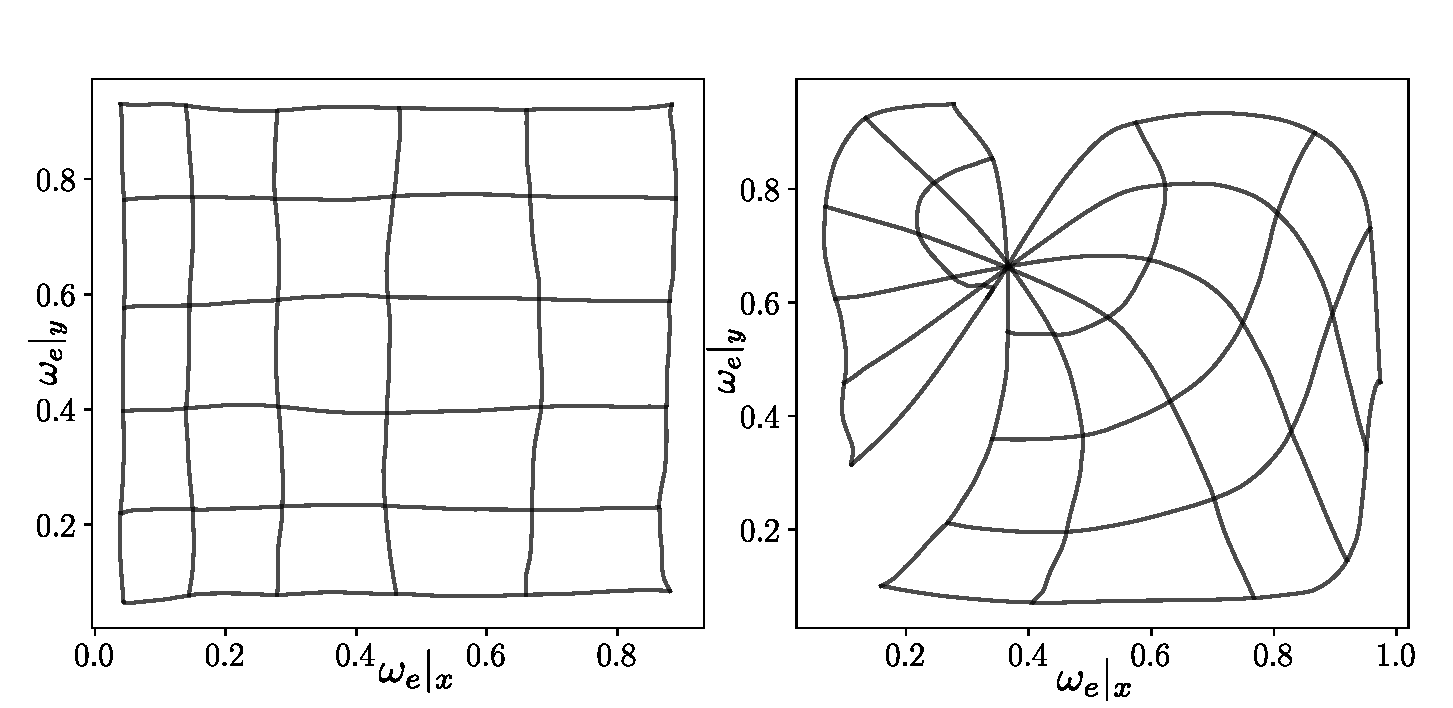
\includegraphics[width=0.7\textwidth]{grid_torsion.pdf}
	\caption{Exemples d'organisations possibles de cartes classiques sur des entrées présentées dans $[0,1]^2$. 
	La carte de gauche est \og bien dépliée \fg{}~: deux entrées proches sont représentées par des BMU proches. 
	Au contraire, la disposition de droite présente un point de torsion. Cette disposition peut évoluer vers une carte bien dépliée ou vers un état stable qui présente encore un point de torsion. Dans ce dernier cas, la carte est toujours organisée sur chaque morceau de carte, mais n'est pas totalement ordonnée. \label{fig:torsion}
	}
\end{figure}

Nous utilisons des architectures de deux cartes 2D, connectées rétroactivement.
Les poids d'une carte sont positionnés sur une grille carrée de taille $100 \times 100$ et indexés entre 0 et 1 sur chaque dimension. Nous notons cet index $\mathbf{p}\m{i} = (p\m{i}|_x, p\m{i}|_y)$.
Chaque carte possède une couche de poids externes $\w\ext$ et une couche de poids contextuels $\w_c$
Les entrées contextuelles sont des positions 2D.
Les activités $a_e$ et $a_c$ sont calculées par une activation gaussienne~:
$$a_e(\mathbf{p},\inpx) = \exp(\frac{||\inpx - \w_e(\mathbf{p}) ||^2}{2\sigma^2})$$
de même pour $a_c$.
La norme utilisée est ici la norme euclidienne, que ce soit dans l'espace d'entrée et dans l'espace des positions de la carte. Les paramètres d'apprentissage (rayons de voisinage et taux d'apprentissage) ne sont pas diminués au cours de l'apprentissage.

La caractérisation de l'organisation dans une carte auto-organisatrice en deux dimensions est plus complexe que dans les cartes en une dimension. En effet, le processus de mise à jour des poids de la carte peut mener à la formation de points de torsion, comme illustré par la figure \ref{fig:torsion}, qui induisent une organisation des poids \og par morceaux \fg{}.
Cette organisation avec des points de torsion préserve bien la continuité des poids dans chaque morceau de la carte. Toutefois, les poids ne sont pas totalement ordonnés à l'échelle de la carte. Ces points de torsions se forment généralement lorsque le rayon de voisinage est trop faible au début de l'apprentissage \parencite{Kohonen1995SelfOrganizingM}.
La présence d'un tel point de torsion pourrait potentiellement affecter l'utilisation de la position du BMU en tant que représentation de l'entrée, car deux entrées proches peuvent avoir un BMU éloigné dans la carte~: la représentation spatiale formée par la position du BMU n'est plus complètement ordonnée. 
Nous ne disposons cependant pas d'éléments permettant de savoir comment une telle cartographie morcelée affecte les capacités d'utilisation de la position du BMU pour l'apprentissage.

Dans les expériences de ce chapitre, nous avons cherché à éviter la formation de tels points de torsion dans les poids externes pour faciliter la compréhension des mécanismes d'organisation.
Pour cela, nous laissons les poids externes s'organiser de façon préalable sur 1000 itérations à partir des activités externes, sans prendre en compte les poids contextuels. Cette pré-organisation est réalisée en prenant un grand rayon de voisinage $r_e = 0.5$.
Ce rayon de voisinage introduit une grande élasticité, ce qui permet de pré-répartir les poids externes sur les entrées externes en évitant de former des points de torsion. 
Après cette étape préalable, nous réduisons le rayon externe à $r_e = 0.2$ et effectuons l'apprentissage des poids externes et contextuels comme décrit dans le modèle CxSOM. Les poids externes affinent alors leur apprentissage. Cette étape ne change pas fondamentalement le comportement des cartes, étant donné que la différence d'échelle entre les rayons externes et contextuels permettait déjà aux poids externes de s'organiser plus rapidement que les poids contextuels.

\subsection{Modèles d'entrées}
\begin{figure}
	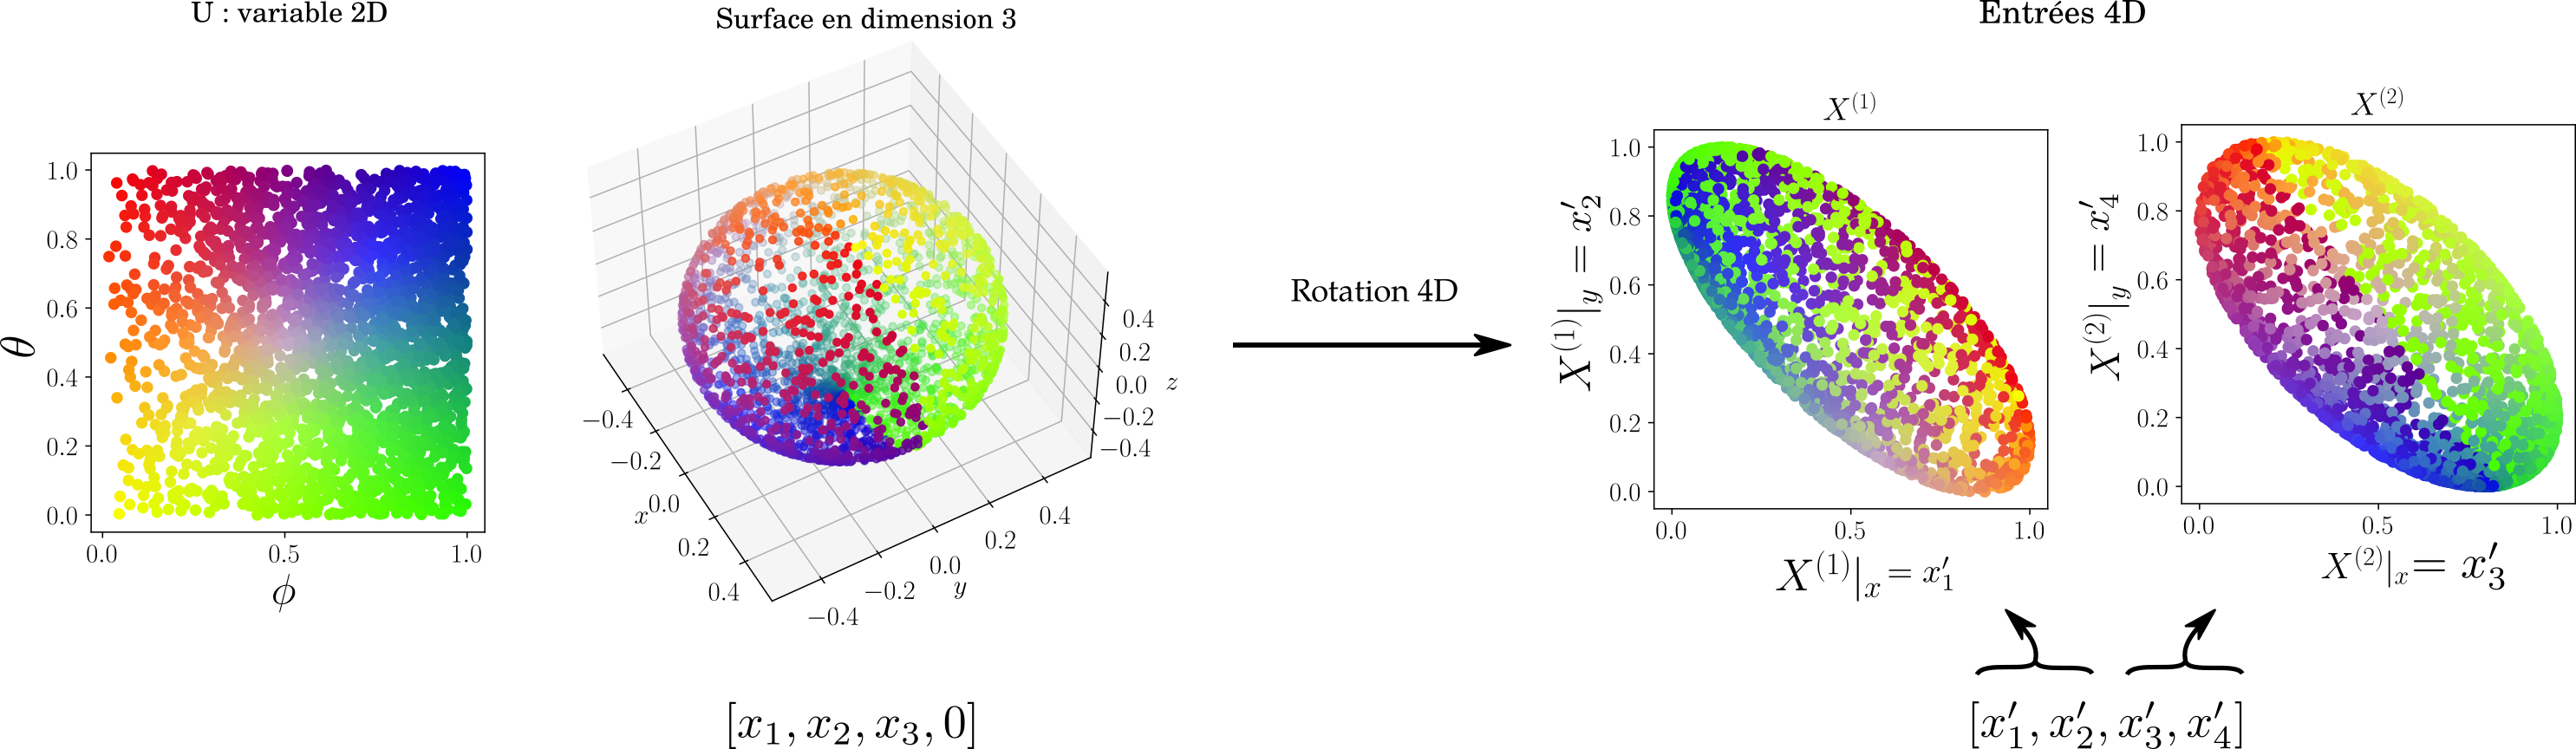
\includegraphics[width=\textwidth]{sphere_inputs_colormap.png}
	\caption{Transformation de la sphère 3D paramétrée par $U$ vers un espace 4D. La rotation permet de répartir les coordonnées des points sur les quatre dimensions sans modifier la structure des entrées. Les modalités sont des valeurs 2D $\inpx\m{1}$ et $\inpx\m{2}$.
	La couleur de chaque point des figures fait référence à la valeur de $U$ correspondante, dont la distribution est présentée à gauche. \`A tout $\inpx\m{1}$ peut correspondre deux valeurs de $U$. Par exemple, $\inpx\m{1} = (0.5, 0.7)$ peut correspondre à $U$ autour de $(0.6,0.3)$ (vert) ou $U$ autour de $ (0.6,0.8)$ (violet).
	\label{fig:sphere_inputs}}
\end{figure}

Nous avons jusqu'à présent utilisé des modèles d'entrées dont chaque modalité $\inpx\m{i}$ comme la variable latente $U$ sont des valeurs 1D.
Afin de complexifier la structure des entrées, nous choisissons d'utiliser des entrées dont chaque modalité est en deux dimensions, et dont le modèle latent $U$ est également 2D.

Nous choisissons comme premier modèle d'entrées des points tirés sur une sphère plongée dans un espace en 4D. 
La structure de ces entrées est illustrée en figure~\ref{fig:sphere_inputs}.
Ces points sont paramétrés par leurs coordonnées polaires $\theta$ et $\phi$. Nous définissons la variable $U$ comme ces angles normalisés sur $[0,1]$.
Pour générer les entrées, nous tirons $U = (\phi,\theta)$ dans $[0,1]^2$ selon la distribution indiquée à gauche de la figure, correspondant à un point sur une sphère en trois dimensions, de coordonnées $(x_1,x_2,x_3,0)$. 
Nous changeons ensuite de repère par une rotation en 4D afin que les coordonnées du point soient distribuées sur les 4 axes de l'espace 4D. Cette rotation s'accompagne d'une translation et d'une mise à l'échelle sur chaque axe afin de normaliser toutes les coordonnées dans $[0,1]$. Le nouvel ensemble de point obtenus $(x_1^\prime,x_2^\prime,x_3^\prime,x_3^\prime)$ sont situés sur une sphère 3D légèrement déformée.
Ces points 4D forment les deux entrées externes en deux dimensions~: $\inpx\m{1} = (x_1^\prime, x_2^\prime)$ et $\inpx\m{2}= (x_3^\prime, x_4^\prime)$.
Sur la figure~\ref{fig:sphere_inputs}, les points sont colorés sur chaque graphique par rapport à la valeur correspondante de $U$, dont la distribution est tracée en figure de gauche.
Une même valeur de $\inpx\m{1}$ peut correspondre à deux valeurs de $U$, ce qui permet de nous placer dans un cas similaire aux entrées tirées sur le cercle, que nous avons utilisées au chapitre~\ref{chap:analyse}.

Nous utiliserons comme second modèle d'entrées 4D des points placés dans l'hypercube $[0,1]^4$. Les deux modalités 2D $\inpx\m{1}$ et $\inpx\m{2}$ sont indépendantes, rappelant la configuration des entrées prises dans le patch $[0,1]^2$ pour des modalités 1D. 
L'étude de configuration d'entrées indépendantes permet d'observer les mécanismes d'organisation qui seraient directement liés aux règles d'apprentissage des cartes.

Nous étudierons enfin une architecture de trois cartes 2D. Les entrées sont tirées sur une sphère, cette fois plongée dans une espace en six dimensions, selon la méthode présentée en figure~\ref{fig:sphere_inputs}. Chaque modalité est en deux dimensions et $U$ est une variable 2D. Dans ce modèle d'entrées, la connaissance de deux modalités sur trois détermine la troisième valeur. Elles nous permettront d'observer la capacité de prédiction d'une architecture de trois cartes 2D.

\subsection{Expériences}

Ce chapitre expose plusieurs observations effectuées sur des architectures de cartes 2D afin de donner un premier aperçu de l'extension aux cartes 2D des propriétés d'organisation observées sur des architectures de cartes 1D.
Les propriétés que nous voulons vérifier sont~:
\begin{itemize}
	\item Les poids externes de chaque carte de l'architecture permettent une bonne quantification vectorielle de leur entrée externe.
	\item Les poids contextuels définissent des motifs pseudo-périodiques, qui forment des sous-cartes organisées sur les valeurs des entrées contextuelles.
	\item Les BMU d'une carte se disposent en zones compactes séparées par des zones mortes. Les BMU encodent à la fois la valeur de l'entrée externe et la valeur du modèle d'entrées $U$. 
	La répartition des valeurs des entrées selon les BMU au sein de chaque carte est effectuée selon deux échelles d'indices.
	\item Une carte ne recevant pas d'entrée externe est capable de générer une bonne prédiction de la modalité manquante dans l'architecture.
\end{itemize}

Nous nous intéressons à la réponse des cartes lors de phases de test, et présentons l'organisation des cartes et de leurs BMU en adaptant les tracés présentés au chapitre~\ref{chap:repr} à des variables en deux dimensions.
Sur les deux modèles d'entrées 4D que nous avons décrits au paragraphe précédent, nous examinerons la disposition des poids externes et contextuels après apprentissage et la disposition des valeurs de $U$ selon la position du BMU. Nous comparerons l'organisation obtenue dans le cas des entrées dépendantes (sphère) et indépendantes (hypercube).
En 1D, le rayon $r_c$ détermine la taille des motifs de poids contextuels. Nous comparerons l'organisation obtenue pour différents rayons de voisinage contextuels et vérifierons la convergence de la relaxation sur ces expériences. Nous observerons enfin la capacité de prédiction d'entrée dans une architecture de trois cartes 2D.

\section{Organisation des cartes sur des entrées présentant une dépendance \label{par:orga2D}}

\subsection{Organisation des poids}

\begin{figure}[h]
	\centering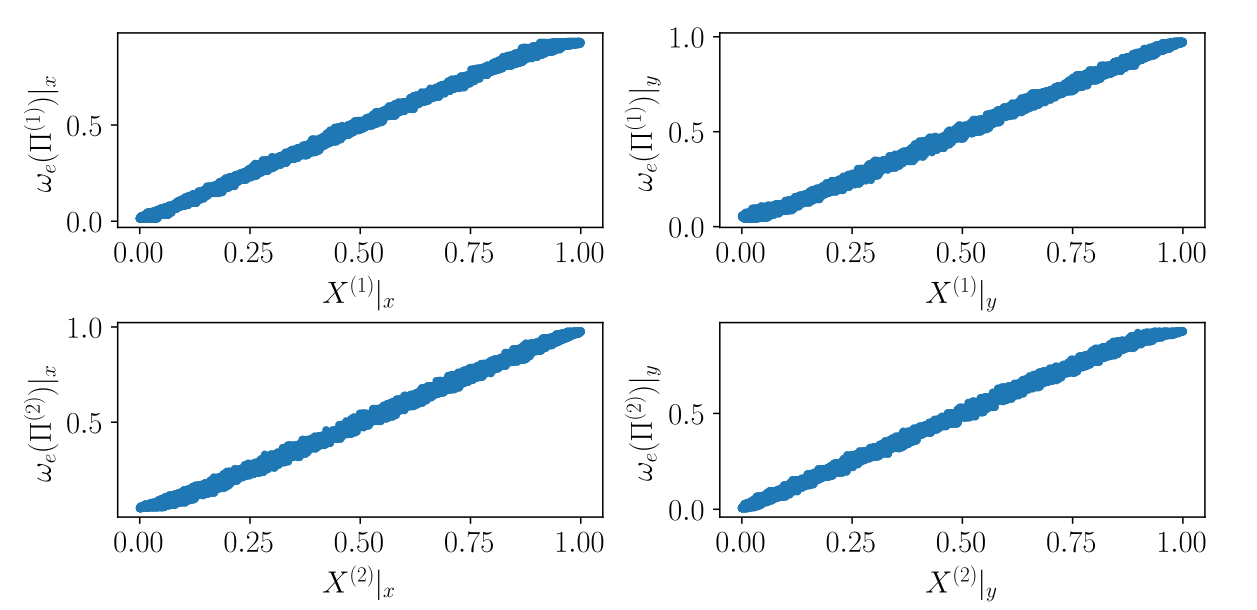
\includegraphics[width=0.8\textwidth]{error-2SOM.png}
	\caption{Erreur de quantification vectorielle sur $\inpx\m{1}$ et $\inpx\m{2}$. $\inpx\m{1}|_x$ et $\inpx\m{1}|_y$ représentent les deux composantes de la valeur 2D $\inpx\m{1}$, de même pour $\inpx\m{2}, \w_e(\bmu\m{1})$ et  $\w_e(\bmu\m{2})$. \label{fig:err_2D}}
\end{figure}

Nous étudions d'abord l'organisation des cartes sur les données tirée sur la sphère, décrite en figure \ref{fig:sphere_inputs}. 
Nous prenons dans cette première expérience les rayons de voisinage à $r_c = 0.02$ et $r_e = 0.2$, qui sont les valeurs des paramètres utilisés pour les cartes 1D.

La figure \ref{fig:err_2D} présente l'erreur de quantification vectorielle réalisée sur chaque entrée. Ces tracés montrent que la quantification vectorielle est correctement réalisée dans chaque carte sur l'entrée externe associée.

La figure~\ref{fig:2som_s_002_wc} présente la disposition des poids externes et contextuels de l'architecture de deux cartes 2D après apprentissage.
En bas, nous représentons les poids externes dans l'espace des entrées~: un n\oe{}ud de la carte est positionné en $\w_e(\mathbf{p})$ qui est une position 2D.
En haut, nous représentons les poids contextuels de la carte sous forme de carte de coloration. Un pixel positionné en position $\mathbf{p}$ est coloré selon la valeur de son poids $\w_c(\mathbf{p})$ qui est une valeur en deux dimensions.


\begin{figure}[h!]
	\begin{minipage}{\textwidth}
	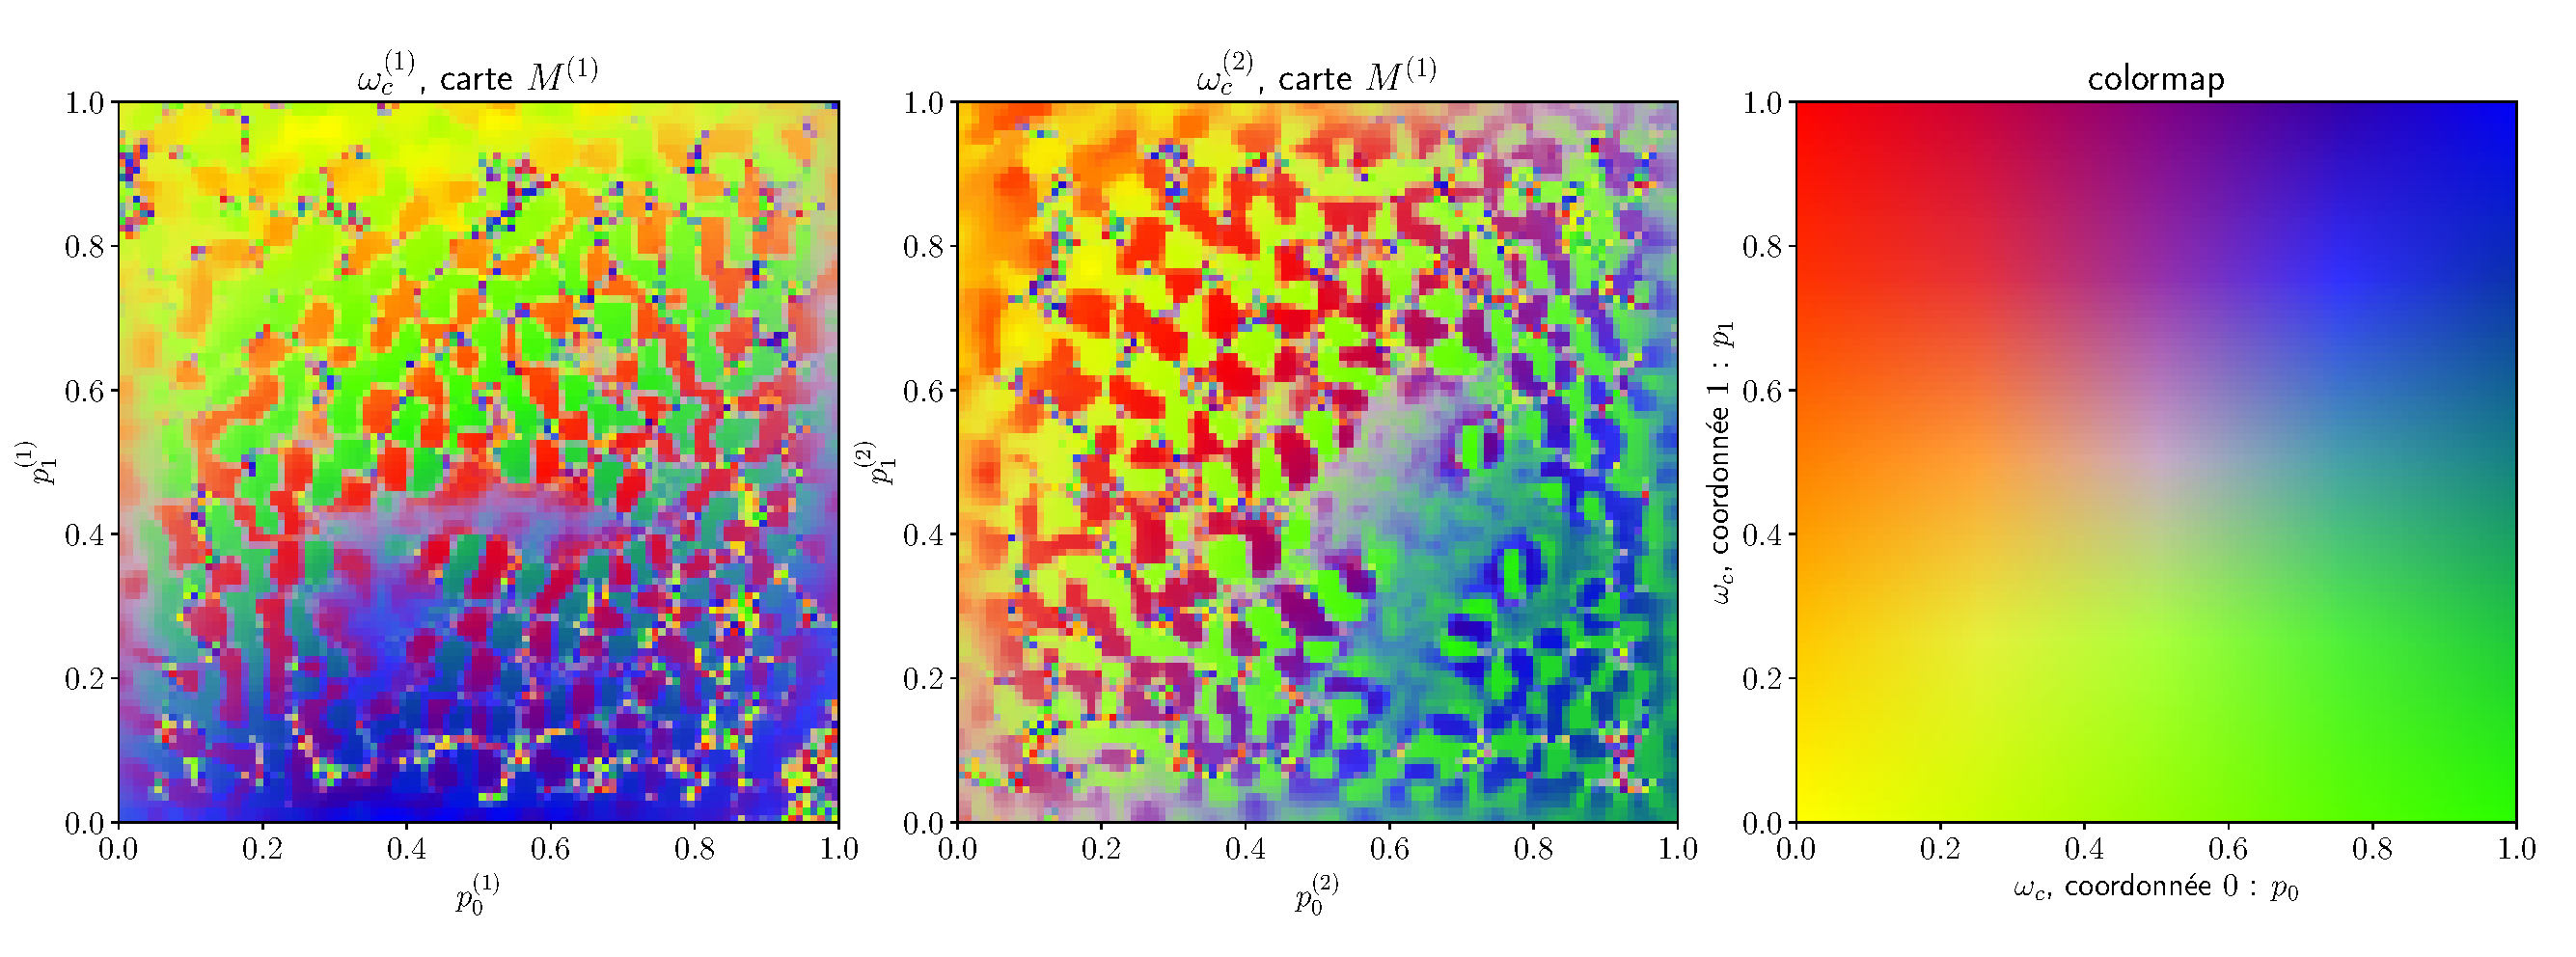
\includegraphics[width=\textwidth]{wc_rc002_afterbug_nopoints.pdf}
	\end{minipage}
	\begin{minipage}{\textwidth}
		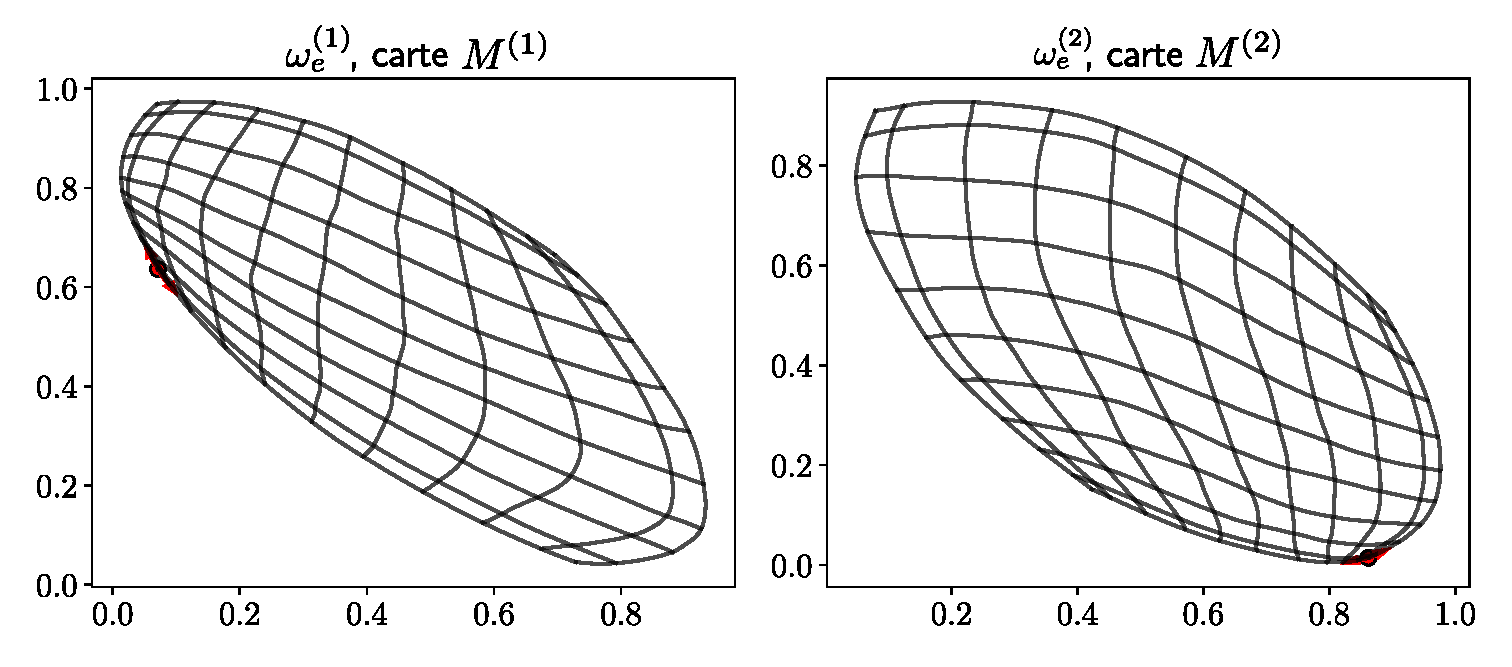
\includegraphics[width=0.7\textwidth]{we_rc002_afterbug_step10.pdf}
		\caption{Tracé des poids externes et contextuels d'une architecture de cartes, organisés sur une sphère dans un espace 4D, avec $r_e =0.2$ et $r_c = 0.02$.
		En bas, les poids externes sont positionnés en fonction de leur valeur $\w_e|_x, \w_e|_y$ et reliés aux n\oe{}uds voisins. Pour une raison de lisibilité, nous avons représenté seulement une partie des connexions, les cartes étant de taille $100 \times 100$. Le coin de position $(0,0)$ de la carte est marqué par le point rouge. Cette représentation permet d'observer directement que les poids externes de chaque carte se déplient sur les entrées externes qui lui ont été présentées, dont on retrouve le tracé en figure~\ref{fig:sphere_inputs}.
		En haut, nous traçons la valeur des poids contextuels. Nous colorons le point situé en position $p|_x, p|_y$ de chaque carte en fonction de la valeur 2D de son poids contextuelles codé par la carte de coloration à droite. Cette représentation fait apparaître une organisation en motifs spatiaux pseudo-périodiques, rappelant le comportement observé en 1D.
		\label{fig:2som_s_002_wc}}
		\end{minipage}
\end{figure}


L'organisation de $\w_e$ montre que chaque carte représente ses entrées externes de la même façon qu'une carte 2D classique~: les poids externes se déplient sur le disque dans lequel sont tirées leurs entrées externes. 
L'organisation de $\w_c$ fait apparaître des motifs oscillant spatialement dans chaque carte, qui rappellent les motifs présents en une dimension, cf. figure~\ref{fig:w}.
Ces motifs pseudo-périodiques sont de taille équivalente et sont répartis sur toute la surface de la carte. 
L'organisation des poids contextuels en motifs se transpose bien des cartes 1D aux cartes 2D. La forme des motifs semble plus variée que sur des cartes 1D, la 2D apportant une dimension supplémentaire à l'organisation.

\subsection{Relation entre $U$ et $\bmu$ \label{par:U_bmu2D}}

\begin{figure}[t]
	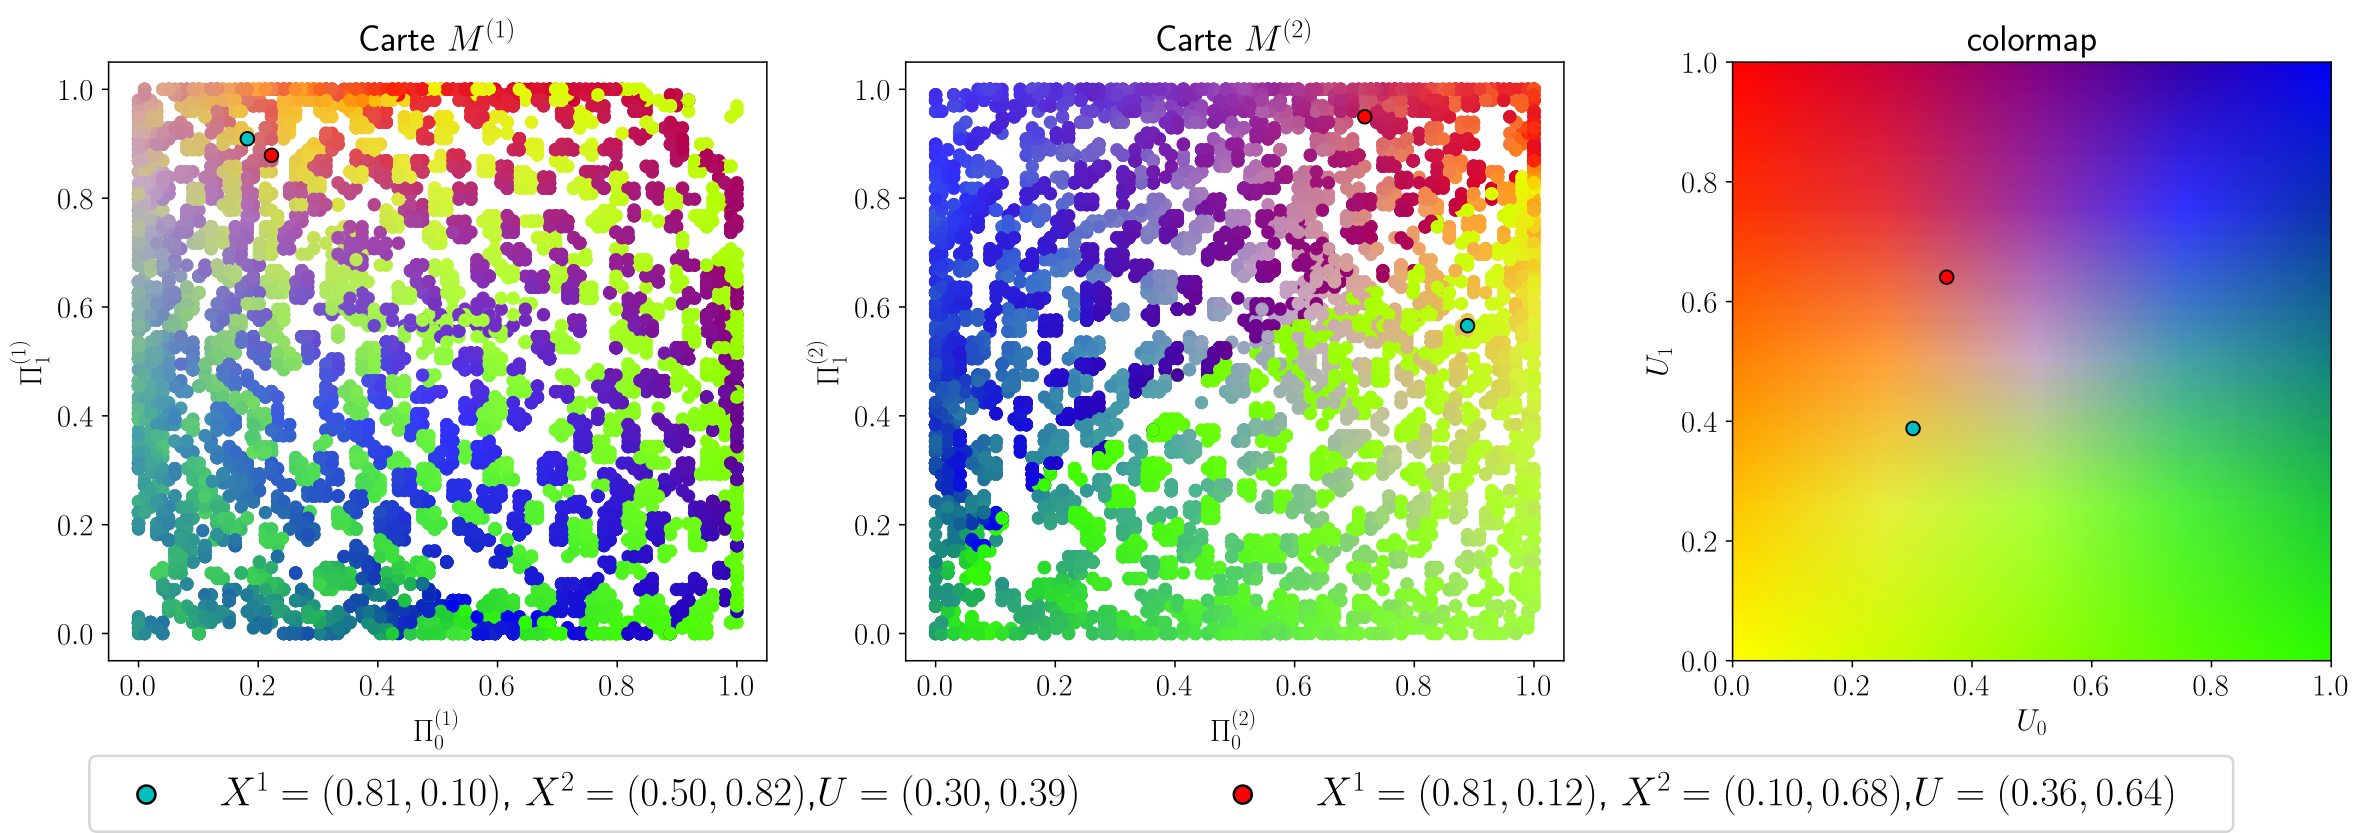
\includegraphics[width=\textwidth]{U_BMU_2SOM_2D.png}
	\caption{Disposition des valeurs de $U$, ici une variable en deux dimensions, selon les valeurs du BMU $\bmu$ dans chaque carte. Les tracés font apparaître que des zones de BMUs se spécialisent pour une valeur de $U$, comme ce qui était observé en une dimension. Les points mis en valeurs en rouge et bleu ont des valeurs très proches d'entrée $X\m{1}$, mais des valeurs différentes pour $U$ et donc $\inpx\m{2}$. Leurs BMU sont positionnés dans deux zones adjacentes sur la carte $M\m{1}$.
	\label{fig:U_BMU}}
\end{figure}

Nous restons dans le cas des entrées tirées sur la sphère plongée en 4D. 
Nous nous intéressons à l'encodage de $U$ et à l'organisation des BMU dans chacune des cartes, dont les poids ont été tracés en figure~\ref{fig:2som_s_002_wc}.
La figure~\ref{fig:U_BMU} représente la valeur de $U$, en couleur, selon la position du BMU $\bmu\m{1}$ et $\bmu\m{2}$ dans chaque carte, sur une étape de test après apprentissage.

Nous constatons que les BMU se regroupent dans des zones distinctes sur la carte. Chaque zone de BMU se spécialise pour une même valeur de $U$. Ces zones semblent séparées par des zones mortes, de tailles variables.
Nous faisons figurer deux points en rouge et bleu sur la figure, qui sont les réponses à deux entrées ayant une valeur de $\inpx\m{1}$ proche, mais une valeur différente de $\inpx\m{2}$ et donc de $U$.
Les BMU de ces deux points sont placés dans deux zones distinctes, mais adjacentes dans la carte $M\m{1}$. Nous retrouvons les deux échelles d'organisation~: l'une s'effectue selon la valeur de l'entrée externe, permettant de choisir le BMU dans une région de la carte. Dans chaque région, le BMU est ensuite différencié selon la valeur de l'autre entrée du modèle.
Ce comportement est ainsi très similaire à celui observé en 1D.
L'organisation des valeurs de $U$ se rapproche également de celle observée en figure~\ref{fig:cr_xp} pour des valeurs de $U$ en une dimension.


Graphiquement, $U$ semble apparaître comme une fonction de $\bmu$ dans chaque carte. Dans le but de vérifier cette relation fonctionnelle, nous avons utilisé le ratio de corrélation. Ses valeurs calculées pour CxSOM et pour les entrées sont présentées dans le tableau \ref{tab:eta2D}. Les ratios de corrélation $\eta(U;\bmu\m{1})$ et $\eta(U;\bmu\m{2})$ sont de $0.98$ dans chaque carte, indiquant que $U$ est proche d'une fonction de $\bmu\m{1}$ et de $\bmu\m{2}$. Cette valeur est supérieure à la relation initiale entre $U$ et chaque modalité $\inpx\m{1}$ et $\inpx\m{2}$, respectivement de $0.81$ et $0.94$, suggérant que les cartes ont créé une relation fonctionnelle qui n'était pas présente dans le modèle d'entrées.
Il est à noter que ces valeurs de ratio de corrélation pour ce modèle d'entrées sont élevées, bien que $U$ ne soit pas une fonction de $\inpx\m{1}$ ou $\inpx\m{2}$. 
Cette observation souligne l'importance de la comparaison de $\eta(U;\bmu)$ à $\eta(U;X)$ pour interpréter correctement sa valeur.

\begin{table}
	\caption{Tableau de comparaison des valeurs de $\eta$ obtenues sur la disposition d'entrées en sphère. \label{tab:eta2D}}
	\centering\begin{tabular}{lcc}
						&$M\m{1}$ 					& $M\m{2}$ 						\\
		Entrées 		& $\eta(U;\inpx\m{1}) = 0.81$ & $\eta(U;\inpx\m{2}) = 0.94$  \\
		CxSOM  	 		& $\eta(U;\bmu\m{1}) = 0.98$ & $\eta(U;\bmu\m{2}) = 0.98$ 	\\
	\end{tabular}
\end{table}

\subsection{Dépendance des motifs de poids contextuels aux paramètres des cartes \label{par:params2D}}

\begin{figure}[ht!]
\begin{minipage}{\textwidth}
	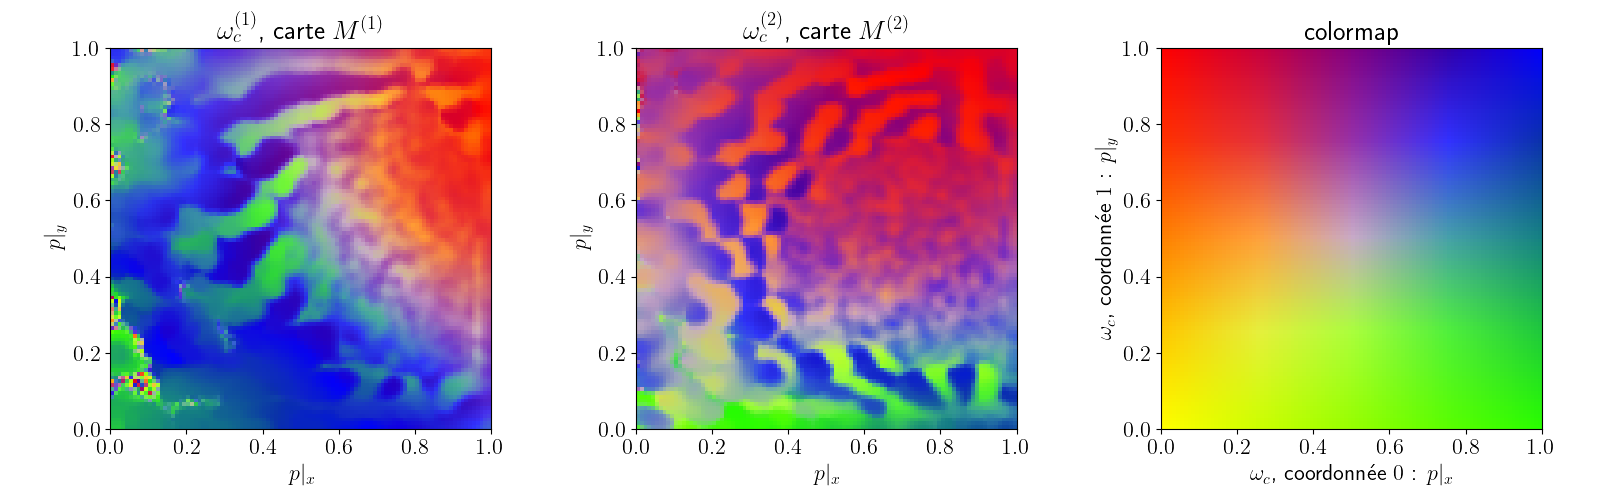
\includegraphics[width=\textwidth]{weights_contexte-0-048_rc003.png}
	\caption{Disposition des poids contextuels après apprentissage, pour $r_e = 0.2$ et $r_c = 0.03$. Les poids forment des motifs pseudo-périodiques, similaires à ceux observés pour $r_c = 0.02$. \label{fig:rc_003}}
\end{minipage}

\begin{minipage}{\textwidth}
	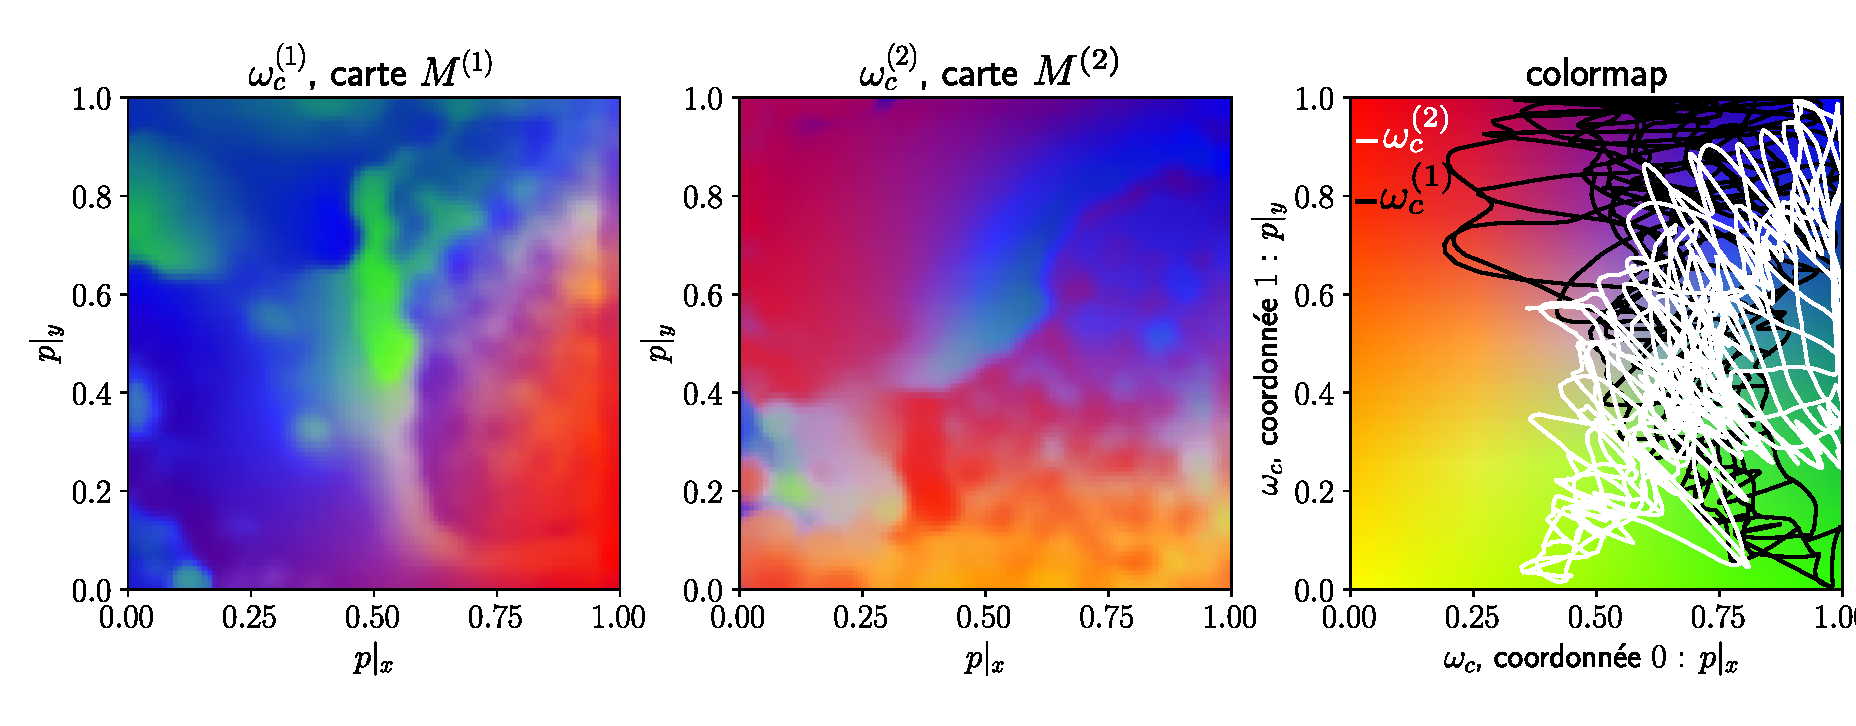
\includegraphics[width=\textwidth]{wc_rc005_grid.pdf}
	\caption{Disposition des poids contextuels après apprentissage, pour $r_c =0.05$. Les poids ne forment pas de motifs. Par ailleurs, nous remarquons que les poids contextuels se déplient sans occuper tout l'espace des positions disponibles, ce qui est mis en évidence par la disposition de la grille, figure de droite ($\w_c\m{1}$ en noir et $\w_c\m{2}$ en blanc).
	Dans cette expérience, nous n'avons pas observé de convergence des poids contextuels~: les poids continuent d'évoluer lentement.
	\label{fig:rc_005}}
\end{minipage}
\end{figure}

En 1D, la formation de motifs de poids contextuels dépend des paramètres de la carte, en particulier du rapport entre les rayons de voisinage.
Nous comparons dans cette section la présence et forme des motifs de poids contextuels pour une même taille de $r_e$, mais des rayons de poids contextuels $r_c$ différents.
Les figures~\ref{fig:rc_003} et \ref{fig:rc_005} présentent la disposition des poids contextuels d'une architecture de deux cartes après apprentissage, avec $r_e = 0.2$ et respectivement $r_c = 0.03$ et $rc = 0.05$. Les entrées sont tirées sur la sphère plongée en 4D.


Nous constatons que les poids contextuels forment des motifs présentant une pseudo-périodicité spatiale pour $r_c = 0.02$ (en figure~\ref{fig:2som_s_002_wc}) et $r_c = 0.03$. La taille de ces motifs dépend de la valeur de $r_c$. Par contre, nous n'observons pas ces motifs pour $r_c = 0.05$.
En 1D, nous avions noté que les zones ne se forment qu'en dessous d'une certaine valeur de $\frac{r_e}{r_c}$ (cf. figure~\ref{fig:rcre}). C'est également ce qui est observé ici, les motifs de poids contextuels apparaissant pour une valeur de $r_c$ se situant entre $r_e = 10 r_c$ et $r_e = 6 r_c$.
Sur la figure~\ref{fig:rc_005}, nous avons également représenté la disposition des poids contextuels sous forme de grille leur espace d'entrées, tracées en figure de droite.
Ces grilles mettent en évidence que les poids contextuels ne se sont pas dépliés sur toutes les positions $[0,1]^2$, ce qui était également observé sur des cartes 1D lorsque $\frac{r_e}{r_c}$ était trop faible.


Enfin, les dispositions de poids contextuels présentées en figures~\ref{fig:2som_s_002_wc} et \ref{fig:rc_003} apparaissent comme des dispositions stables de poids~; nous avons constaté graphiquement cette stabilité. Au contraire, la configuration présentée en figure~\ref{fig:rc_005} n'est pas une configuration stable. Nous avons observé sur cette expérience une dérive lente des poids contextuels au cours des itérations, qui gardent toutefois une structure générale semblable à celle représentée sur la figure.

Nous pouvons conclure de ces observations préliminaires sur des exemples de cartes en deux dimensions que la formation de motifs de poids contextuels est un mécanisme qu'on retrouve dans des cartes 1D comme des cartes 2D.
Ces motifs dépendent du rapport entre rayons de voisinage externe et contextuels.
Comme sur les cartes 1D, nous observons que les BMU forment des zones sur la carte et se spécialisent pour une valeur du modèle d'entrée et non seulement de l'entrée externe.
L'aspect 2D apporte beaucoup moins de contraintes sur la forme des zones que sur des cartes en une dimension, diversifiant les motifs de poids contextuels.


\subsection{Convergence de la relaxation \label{par:conv2D}}

Nous voulons vérifier que la relaxation converge lors des expériences présentées dans ce chapitre, afin de s'assurer que les BMU trouvés correspondent bien à un maximum d'activité dans chaque carte et ont donc un sens de \og Best Matching Unit \fg{}.
Nous traçons en figure \ref{fig:relax2D} l'évolution du taux de convergence des tests et du nombre moyen de pas de relaxation au cours de l'apprentissage, selon la méthode présentée au chapitre \ref{chap:relaxation}. Le taux de convergence correspond au pourcentage d'observations n'ayant pas mené à une convergence lors de chaque phase de test~; le nombre moyen de pas de relaxation est calculé sur chaque phase de test.
On considère que la relaxation n'a pas convergé si le nombre de pas atteint le seuil maximal de $\tau_{max} = 1000$ pas fixé par notre étude. Le nombre moyen de pas de relaxation observé étant de 20 pas, 1000 pas est un seuil que nous jugeons pertinent pour considérer que la relaxation n'a pas convergé.
Nous traçons ces évolutions pour les différentes configurations de paramètres de cartes~: nous avons réalisé trois expériences de mêmes paramètres $r_e=0.2$ et $r_c = 0.02$, une expérience avec $r_c = 0.03$ (figure~\ref{fig:rc_003}), et une avec $r_c = 0.05$ (figure \ref{fig:rc_005}).
Dans cette dernière expérience, les poids n'ont pas formé de zones distinctes.


Nous observons sur ce tracé que la relaxation converge bien dans entre 95 et 98 \% des cas tout au long de l'apprentissage, ce qui indique que le BMU trouvé par relaxation a bien un sens de maximum d'activation dans la majorité des tests (voir chapitre~\ref{chap:relaxation}).
Les valeurs des indicateurs trouvées pour $r_c = 0.05$ sont similaires au cas $r_c = 0.02$, dans lequel les poids ont bien convergé. La relaxation dans des cartes en deux dimensions n'est donc pas particulièrement liée à la formation de motifs stables dans les poids~: la relaxation semble trouver un point de convergence dans un cas général de cartes en 2D. Cette observation est prometteuse pour la construction d'architectures de cartes 2D.

\begin{figure}
	\centering
	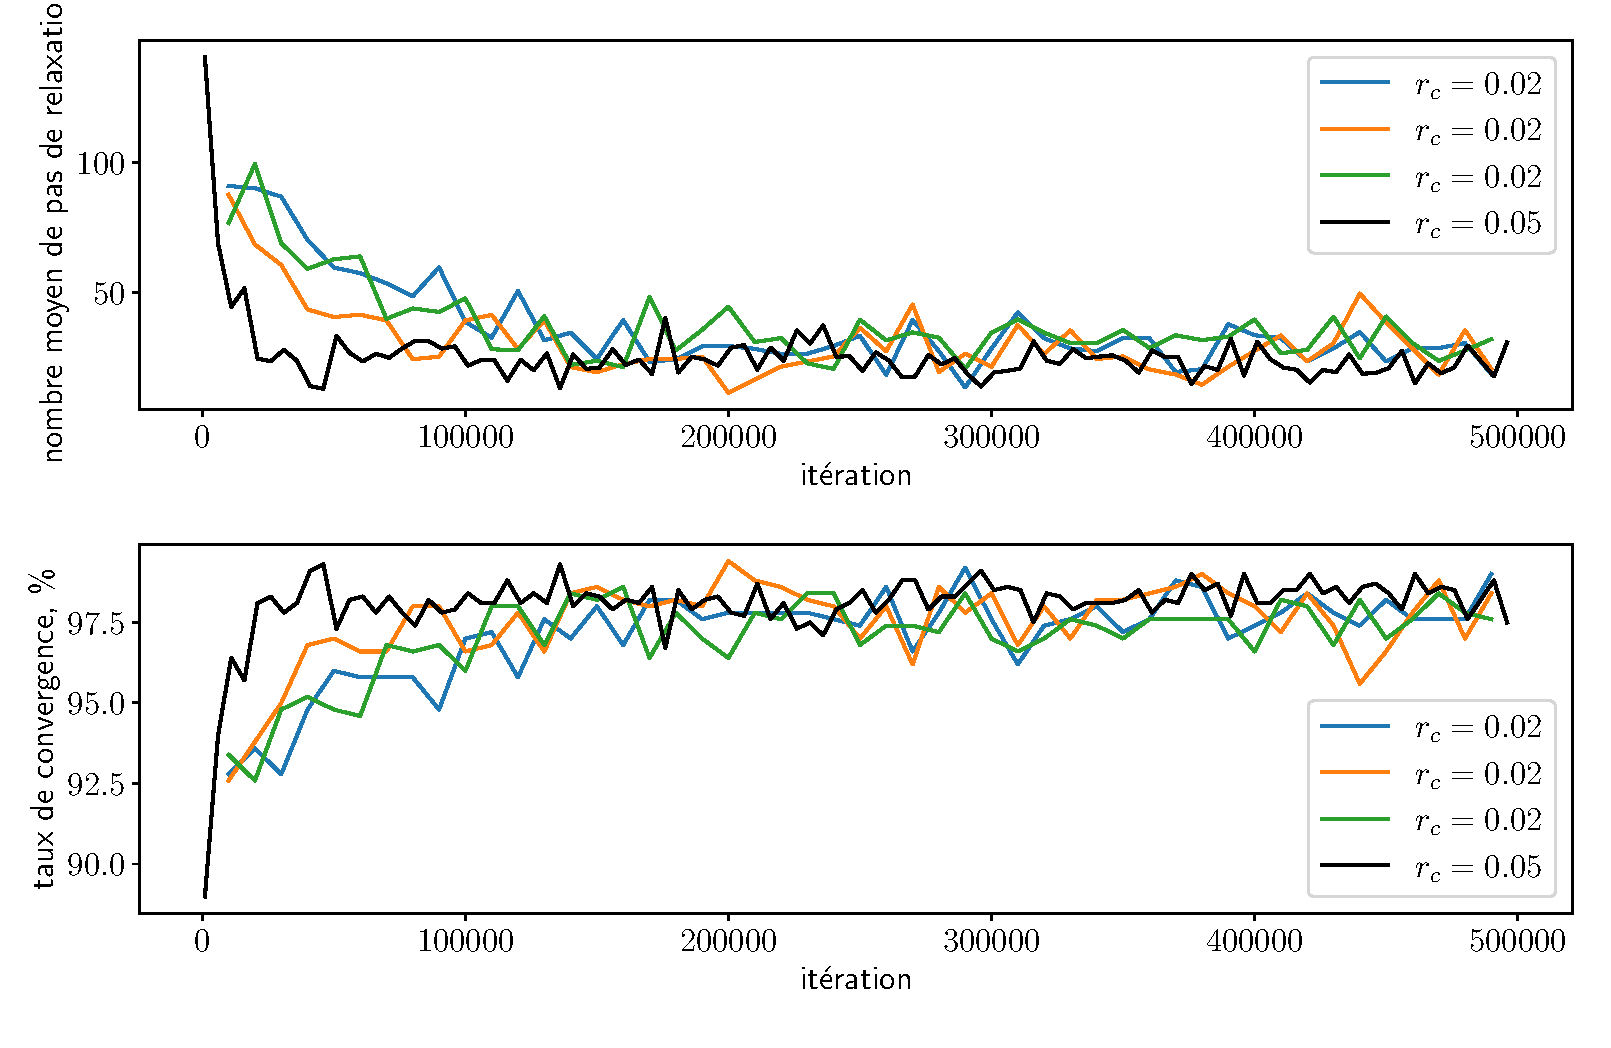
\includegraphics[width=0.8\textwidth]{conv_relax_2maps.pdf}
	\vspace{-0.5cm}
	\caption{\'Evolution de la convergence de la relaxation au cours de l'apprentissage. Nous avons réalisé les tracés sur plusieurs expériences générées pour différents paramètres d'apprentissage. Les entrées sont tirées sur la sphère plongée en 4D. 
	La relaxation converge dans plus de 95 \% des cas en fin d'apprentissage~: la valeur trouvée à l'issue de la relaxation correspond à une position maximisant l'activité dans chaque carte, quels que soient les motifs de poids contextuels créés par les cartes. \label{fig:relax2D}}
\end{figure}

\section{Organisation des cartes sur des entrées indépendantes \label{par:cub2D}}

Nous nous intéressons enfin à l'organisation d'une architecture de deux cartes prenant des entrées $(\inpx\m{1}, \inpx\m{2}) \in [0,1]^2 \times [0,1]^2$ indépendantes.
Nous avons observé la formation de motifs de poids contextuels sur des cartes en deux dimensions lorsqu'elles apprennent les entrées tirées sur la sphère. Nous voulons observer si ces motifs se créent également dans le cas où les deux entrées externes sont indépendantes.
D'après les comportements observés sur des cartes 1D, nous nous attendrions à ce que chaque carte présente des zones, dans lesquelles les poids contextuels forment une sous-carte de tout $[0,1]^2$.
Les rayons de voisinage sont pris à $r_e = 0.2, r_c = 0.02$.

Les valeurs des poids externes et contextuels obtenus après apprentissage sont tracés en figure \ref{fig:2som_cub_wc}.
Les poids externes sont bien dépliés sur l'ensemble des entrées, ce qui est similaire au cas en une dimension.
Les poids contextuels restent par contre centrés autour de $0.5$, mis en évidence par les tracés en blanc et noir sur la carte de coloration à droite de la figure.
Pourtant, nous avons observé que toutes les positions d'une carte ont bien été BMU lors des phases de tests.

Ce comportement de moyennage est à rapprocher du comportement limite observé sur une architecture de 10 cartes en une dimension (cf. figure~\ref{fig:bigdim})~: nous avons observé qu'une architecture de 10 cartes apprenant sur 10 entrées 1D indépendantes voient également leurs poids contextuels se moyenner autour de $0.5$ dans chaque carte.
Les connexions entre les n\oe{}uds semblent ici trop rigides pour permettre aux poids contextuels de se déplier sur tout le carré dans chacune des zones. Ils prennent donc une valeur moyenne.
Le comportement de moyennage est finalement présent sur des architectures de cartes 1D comme 2D, et semble être renforcé sur les cartes en deux dimensions, car ce mécanisme est observé sur une architecture de seulement deux cartes.

Ce comportement peut apparaître comme une limite de CxSOM, marquant le fait que les poids contextuels manquent de liberté pour s'organiser. Cette limite sera à nuancer en fonction des paramètres d'apprentissage (rayons de voisinage, taille des cartes, taux d'apprentissage), qui n'ont pas été soumis à une optimisation dans cette étude.
Au contraire, nous pouvons aussi envisager ce comportement comme une capacité de détection de dépendance entre entrées, qui serait encore plus marquée sur les cartes 2D que sur les cartes 1D. 

\begin{figure}
	\centering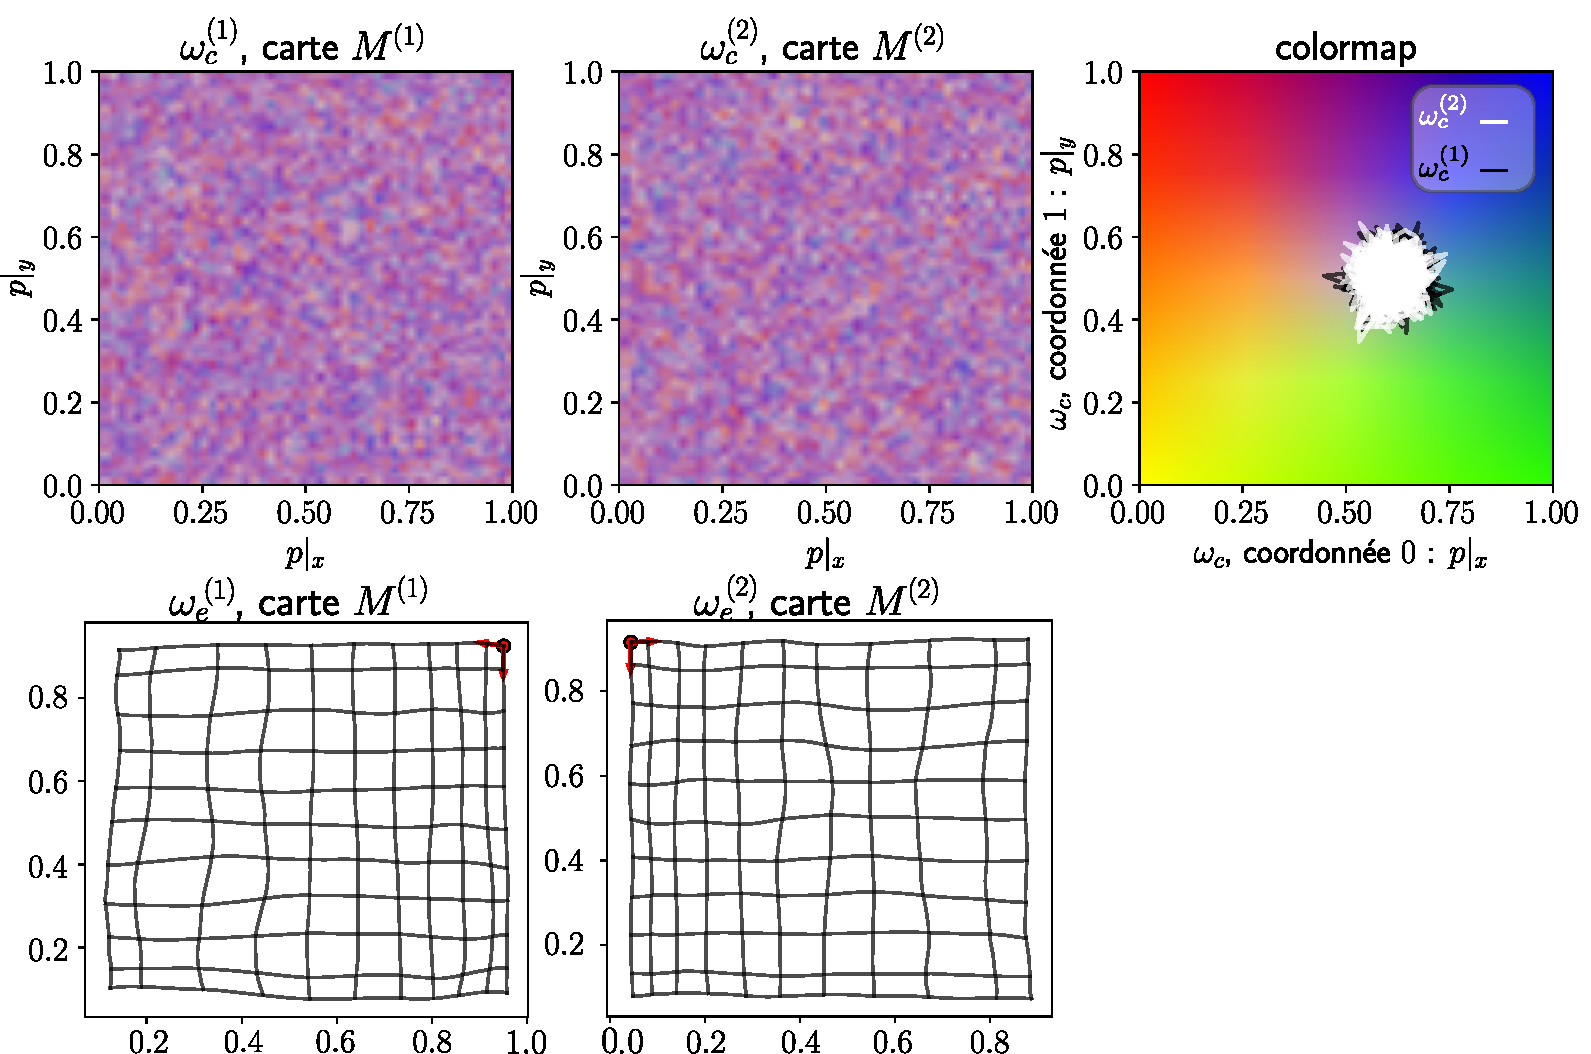
\includegraphics[width=\textwidth]{w_cub_rc002.pdf}
	\caption{Poids des cartes $M\m{1}$ et $M\m{2}$ après 200000 itérations d'apprentissage sur les entrées indépendantes. Les poids contextuels, en haut, sont tracés en carte de coloration~; les poids externes, en bas, sont tracés dans l'espace des entrées.
	Nous constatons que les poids contextuels ne se déplient pas sur toutes les valeurs prises par les BMU et restent centrés vers le milieu de la carte. \label{fig:2som_cub_wc}}
\end{figure}

\section{Prédiction d'entrée \label{par:pred2D}}

\begin{figure}
	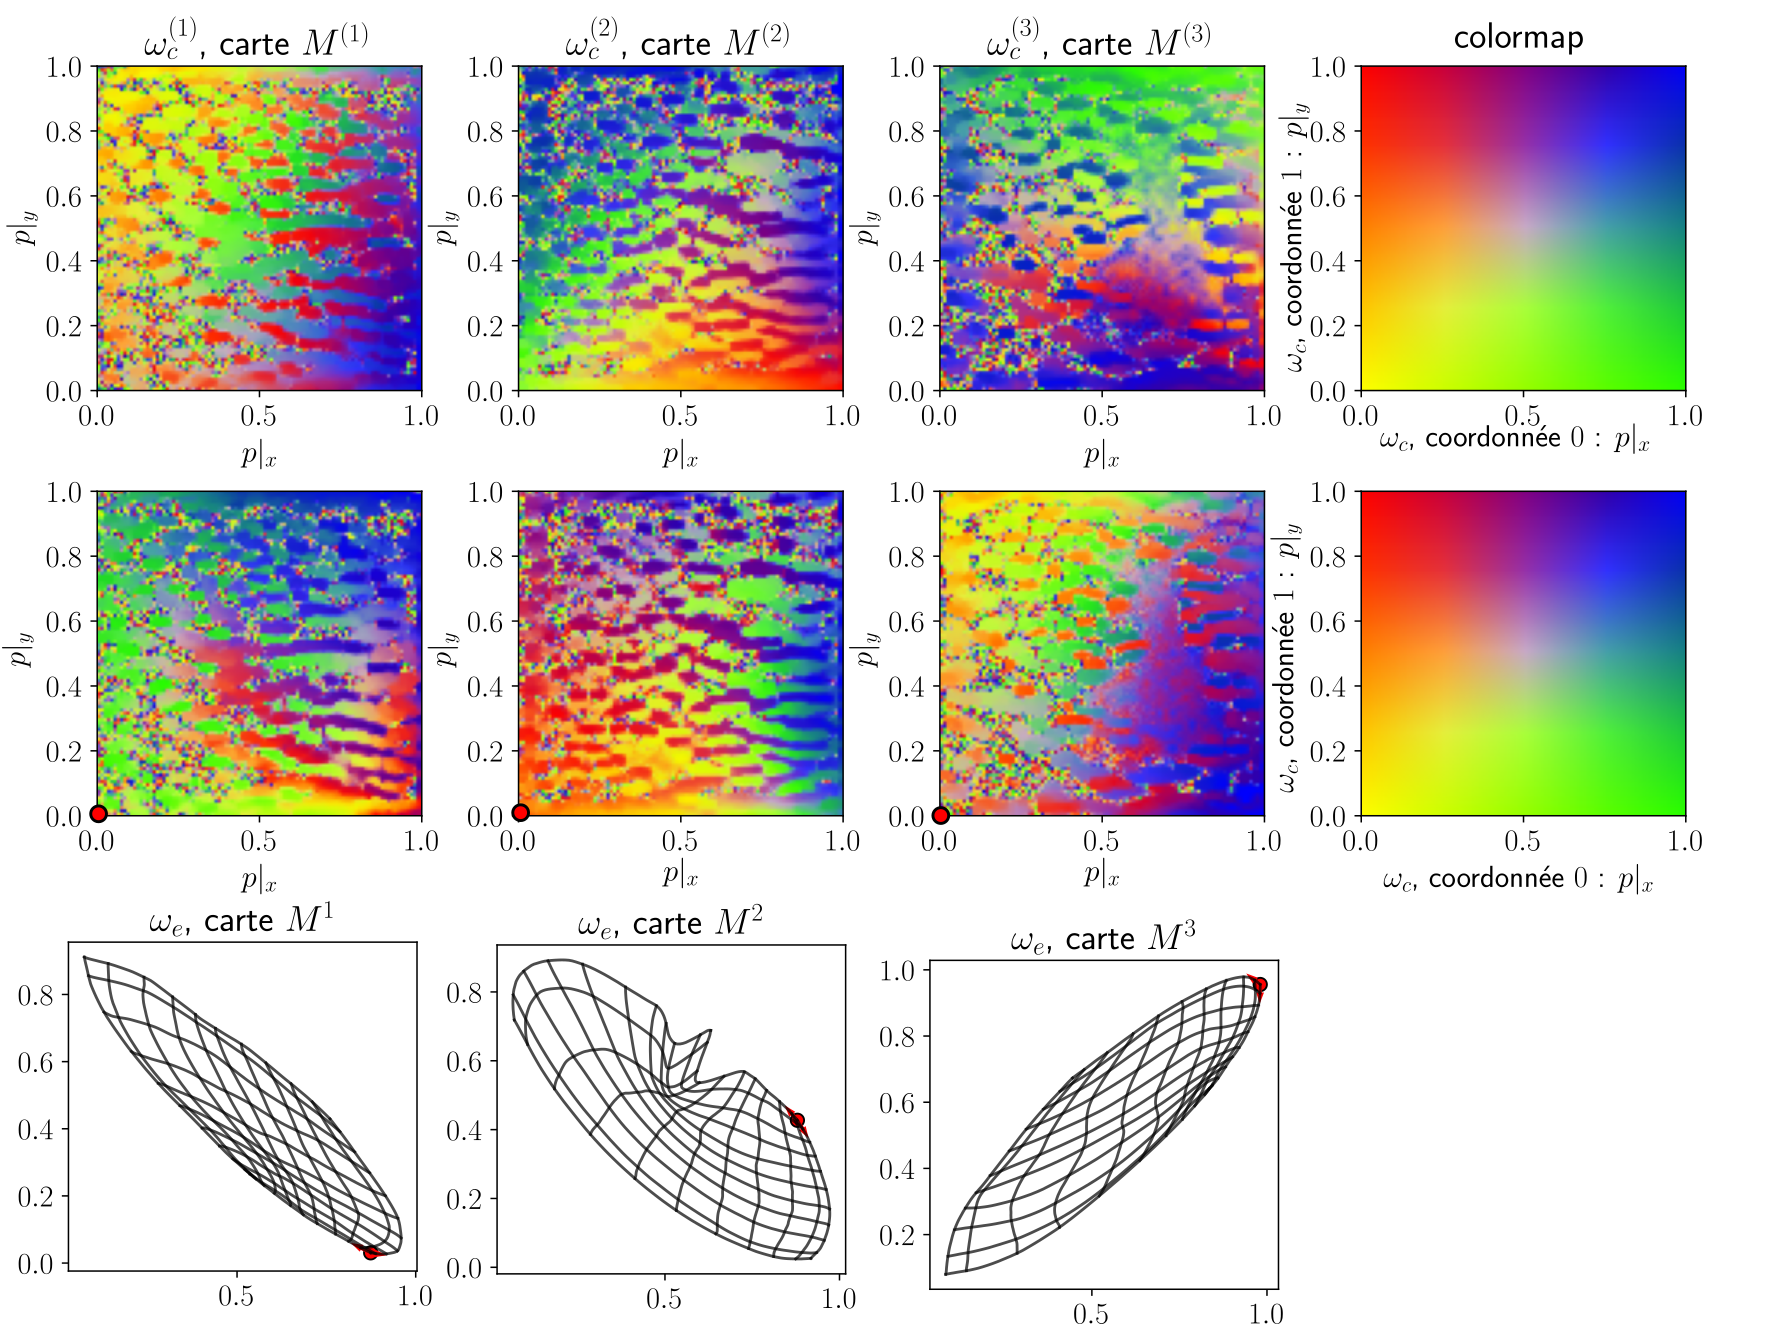
\includegraphics[width=\textwidth]{3SOM_S_wc_239999.png}
	\caption{Tracés des poids externes dans l'espace des entrées (en bas) et des deux couches de poids contextuels de chaque carte sous forme de carte de coloration (en haut). Les motifs formés par les poids contextuels sont similaires à ceux observés sur deux cartes. \label{fig:3som_w}}
\end{figure}

Nous avons constaté un parallèle entre l'organisation des cartes 1D et 2D. Nous avons également observé que la relaxation converge correctement dans les architectures de cartes 2D étudiées, traduisant que la dynamique de relaxation permet de trouver un BMU correspondant bien à un maximum d'activation dans chaque carte.
Nous nous attendons donc à ce qu'une architecture de cartes 2D soit en mesure de générer la prédiction d'une entrée manquante.

Nous vérifions cette capacité de prédiction sur une architecture de trois cartes en deux dimensions. 
Les entrées externes sont tirées sur une sphère de dimension 3, plongée dans l'espace en 6D par le même processus de rotation qu'en 4D (figure~\ref{fig:sphere_inputs}). $U$ est ici toujours une variable $2D$. 
Dans cette configuration, la connaissance de deux entrées sur trois et du modèle détermine la troisième, ce qui permet d'envisager une prédiction.
Nous prenons $r_e = 0.2$ et $r_c = 0.02$ et des cartes de taille $100 \times 100$. Les cartes ont été entraînées sur 250 000 itérations, à l'issue desquelles les poids externes et contextuels ont atteint une position stable.

Nous traçons les poids externes et contextuels des trois cartes en figure~\ref{fig:3som_w}.
L'organisation des poids contextuels conduit à la présence de motifs très semblables à ceux observés sur une architecture de deux cartes.
Nous réalisons une étape de prédiction à la fin de l'apprentissage lors de laquelle une carte ne reçoit plus d'entrée externe, ici $M\m{2}$~; la valeur de $\w\ext\m{2}(\bmu\m{2})$ est utilisée comme prédiction de l'entrée $\inpx\m{2}$.
La figure~\ref{fig:3som_pred} représente l'erreur de prédiction sur $\inpx\m{2}$.
Les valeurs de $\inpx$ et $\w_e$ étant 2D, nous avons représenté séparément chaque dimension. 
Nous constatons que les valeurs prédites sont proches des valeurs théoriques, suggérant que l'architecture a correctement appris le modèle des entrées 2D.
L'erreur de prédiction est plus élevée que l'erreur de quantification réalisée dans les deux autres cartes, ce qui n'était pas le cas en 1D.
Par ailleurs, chaque carte possède 10000 n\oe{}uds~: on s'attendrait à une meilleure capacité de prédiction. Toutefois, cette capacité de prédiction observée dans une architecture de cartes 2D reste prometteuse et devra être mise en perspective grâce à une optimisation plus poussée des paramètres d'apprentissage de l'architecture.

Nous pouvons néanmoins noter que l'organisation induite par le modèle CxSOM présente de nombreux n\oe{}uds inutilisés en 1D comme en 2D, les n\oe{}uds morts. Ces n\oe{}uds sont utiles pour l'organisation en tant que zones de transition, mais n'encodent pas de valeur pour la quantification vectorielle de l'entrée externe et la prédiction. Ces n\oe{}uds morts sont beaucoup plus nombreux dans les cartes 2D que les cartes 1D car ils s'étendent sur les deux dimensions. On a donc globalement une fuite massive d'unités d'encodage dans le modèle CxSOM. 
Cela pourrait expliquer le fait que la prédiction est assez mal réalisée en 2D~: une faible proportion de n\oe{}uds, sur les 10000 que possède la carte, encodent véritablement les valeurs d'entrées.


\begin{figure}
\centering\includegraphics[width=0.8\textwidth]{3SOM_error_closed.pdf}
\caption{Tracé de l'erreur de prédiction $\w_e\m{2}(\bmu\m{2})$ en fonction de la valeur théorique de $X^{(2)}$, non présentée à l'architecture, dans une architecture de trois cartes 2D prenant des entrées $X^{(i)}$ en deux dimensions $[X^{(i)}|_x, X^{(i)}|_y]$. Nous traçons sur une ligne, pour chaque entrée, les dépendances entre chacune des dimensions
lorsque la carte $M^{(2)}$ ne reçoit pas d'entrée externe. Les cartes $M^{(1)}$ et $M^{(3)}$ ayant une activité externe, le graphique montre que la quantification vectorielle est bien réalisée dans ces cartes. La carte $M^{(2)}$ est uniquement activée par les connexions contextuelles venant de $M^{(1)}$ et $M^{(3)}$. La figure centrale montre que la prédiction est correctement réalisée, mais que l'erreur de prédiction est assez élevée. \label{fig:3som_pred}}
\end{figure}

\section{Conclusion}

Les expériences proposées dans ce chapitre donnent une première idée des comportements que l'on peut attendre des architectures de cartes en deux dimensions.
Pour cette analyse, nous nous sommes appuyée sur la méthode d'étude de carte proposée tout au long de cette thèse.
Nous nous sommes intéressée à des architectures de deux et trois cartes 2D, apprenant des modalités 2D. Le modèle d'entrées prises sur une sphère est un pendant en 4D du modèle d'entrées 1D prises sur le cercle. Dans ce modèle, chaque valeur de $\inpx\m{1}$ ainsi que chaque valeur de $\inpx\m{2}$ peut correspondre à deux valeurs de $U$

Nous avons d'abord observé que l'émergence de motifs pseudo-périodiques de poids contextuels est une propriété qui se transpose des cartes 1D aux cartes 2D. 
La formation de ces motifs apparaît permettre d'encoder la valeur du modèle d'entrées $U$ au sein de chaque carte. Nous avons constaté que $U$ est une fonction du BMU dans chacune des cartes, ce qui est correctement évalué par le ratio de corrélation.
Les motifs de poids contextuels dépendent du rapport entre les rayons de voisinage externes et contextuels et ne se forment qu'à partir d'une certaine valeur de ce rapport.
Sur les expériences que nous avons réalisées, la relaxation converge en fin d'apprentissage et le BMU des cartes 2D a donc un sens de maximum d'activation dans une carte. Enfin, nous avons observé une capacité de prédiction satisfaisante d'une modalité manquante sur une disposition d'entrée en sphère dans un espace 6D.
L'architecture de cartes en deux dimensions étudiée présente ainsi des propriétés similaires à celles observées sur les cartes 1D et généralise le comportement observé en 1D, ce qui est prometteur pour la construction d'architectures de cartes 2D. Le passage de 1D à 2D apporte une diversité dans les comportements d'organisation relevés sur les cartes~: la forme des motifs spatiaux formés par les poids contextuels est plus variable que dans le cas des cartes en une dimension.
Les paramètres des architectures ont été fixés à partir des paramètres utilisés en une dimension. L'étude des cartes de Kohonen classique et les comportements variés observés dans ce chapitre motivent une meilleure étude paramétrique des architectures de cartes, qui pourra permettre d'améliorer les comportements d'organisation et de prédiction que nous avons observés.

% Notons que comportement de moyennage observé sur le modèle d'entrées en hypercube soulève des interrogations quant à la capacité des cartes à apprendre des modèles d'entrées dans lesquels $U$ est de grande dimension. 
% Par ailleurs, le passage aux cartes 2D s'accompagne de beaucoup plus de n\oe{}uds morts qu'en 1D, soit une fuite d'unités servant à l'apprentissage.
% Ces deux observations rejoignent le questionnement que nous avons émis à propos des cartes 1D~: est-il possible d'encoder les relations entre les entrées dans l'architecture sans trop dégrader la capacité d'apprentissage des entrées externes~?



\ifSubfilesClassLoaded{
    \printbibliography
    %\externaldocument{../main.tex}   
}{}
\end{document}



% PLAN


% Convergence des poids :
% - Dépend des paramètres, contrairement à la carte en 1D on n'arrive pas forcément dans une position stable
% - Rc = 0.02 : point fixe, avec une partie 
% - Chaque expérience différente : grande dépendance aux conditions initiales. 